\chapter{Materials and Methods}
\section{Simulation System Overview}
The network environment to be created for this thesis is realistic using GNS3 and closely analyzed for DDoS attacks. The setup entails the use of Fedora Linux as the main host machine, hosting web server, GNS3 software, other virtual features such as Cisco routers, Ethernet switches, virtual personal computers among others. The following sections describe the key components of the simulation system in detail:
\begin{table}[h]
    \centering
    \begin{tabular}{|c c|}
    \hline
        Operating system & Ubuntu Linux \\
    \hline
        CPU & 2 virtual Processors \\
    \hline
        Memory & 4GB RAM \\
    \hline
        Storage & 25GB \\
    \hline
        Application & Apache Webserver \\
    \hline
    \end{tabular}
    \caption{Victim's hardware details}
    \label{tab:my_label}
\end{table}
\begin{table}[h]
    \centering
    \begin{tabular}{|c c|}
    \hline
        Operating system & Kali Linux \\
    \hline
        CPU & 2 virtual Processors \\
    \hline
        Memory & 2GB RAM \\
    \hline
        Storage & 15GB \\
    \hline
    \end{tabular}
    \caption{Attacker's hardware details}
    \label{tab:my_label}
\end{table}
\begin{table}[h]
    \centering
    \begin{tabular}{|c c|}
    \hline
        Operating system & Ubuntu Linux \\
    \hline
        CPU & 2 virtual Processors \\
    \hline
        Memory & 2GB RAM \\
    \hline
        Storage & 15GB \\
    \hline
    \end{tabular}
    \caption{Botnets' hardware details}
    \label{tab:my_label}
\end{table}
\\
\section{Network Components}
The network topology in the simulation includes a Cisco C3745 router, generic Ethernet switches, and multiple virtual PCs. These components are interconnected to emulate a typical enterprise or service provider network:
\begin{itemize}
    \item Cisco C3745 Router
    \\ Serves as the central routing device, managing traffic between different network segments. Configured with realistic routing protocols, such as OSPF or EIGRP, to mimic real-world scenarios.
    \item Generic Ethernet Switch
    \\ Acts as a layer 2 intermediary device to interconnect virtual PCs and route traffic to the router. Provides a realistic simulation of how network switches handle traffic in modern network infrastructures.
    \item Virtual PCs
    \\ Represent client devices that simulate legitimate and malicious traffic. Used to generate normal user traffic as well as DDoS attack traffic.
    \item GNS3 Network Emulator
    \\ The entire network is orchestrated using GNS3, a versatile tool for designing and testing complex network topologies in a virtual environment.
    \item Topology Design
    \\ A centralized topology is built, with the web server connected to the Cisco C3745 router via Ethernet switches, and multiple virtual PCs distributed across different subnets. 
    \item Performance Monitoring and Logging
    \\ To analyze the impact of DDoS attacks and validate the effectiveness of mitigation strategies, the simulation includes performance monitoring tools:
\end{itemize}
\subsection{Simulation Features}
GNS3 allows real-time monitoring of network traffic and performance metrics during the simulation. Integrated tools such as Wireshark provide detailed packet analysis, enabling in-depth evaluation of DDoS attack behaviors and mitigation techniques.
\subsection{Monitoring Tools}
Wireshark: Used for packet capture and analysis, identifying anomalies and traffic patterns during the attack.
\\
System Resource Monitoring: The Ubuntu host system is monitored for CPU, RAM, and network bandwidth utilization to measure the impact of DDoS attacks on server performance.
\\
Log Analysis: Web server logs are reviewed to track request patterns, detect abnormal traffic, and quantify the attack scale.
\section{Connection set up}
\begin{figure}[htp]
    \centering
    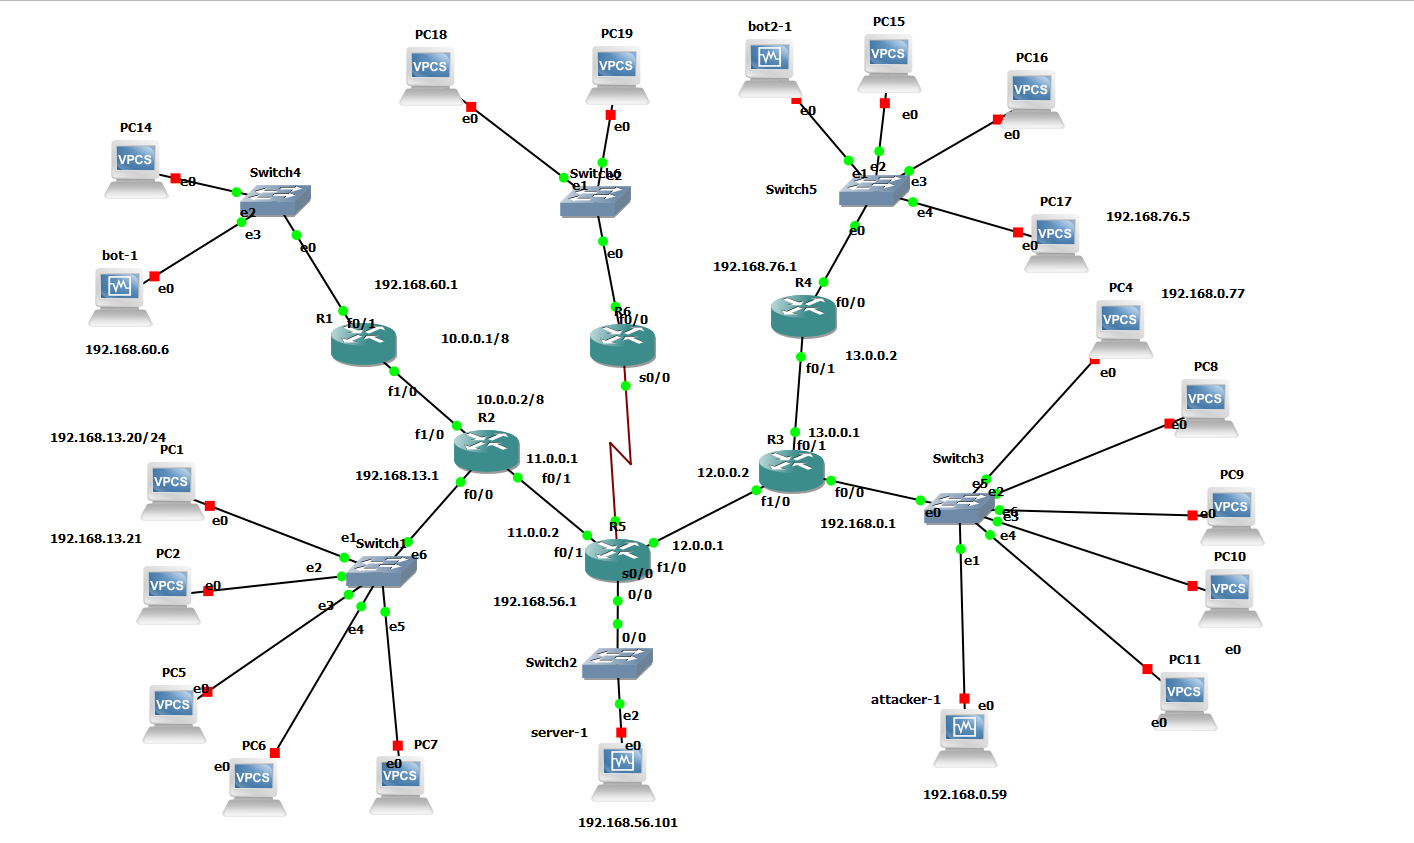
\includegraphics[width=0.8\linewidth]{thesis/NetworkSimulation.png}
    \caption{Network Simulation}
    \label{fig:enter-label}
\end{figure}
\begin{figure}[htp]
    \centering
    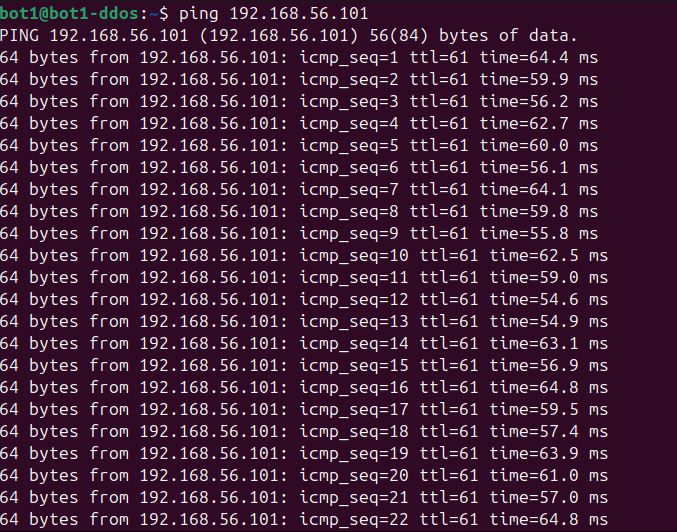
\includegraphics[width=0.7\linewidth]{thesis/bot1ToServer.png}
    \caption{Ping to check connection between bot1 and server}
    \label{fig:enter-label}
\end{figure}
\begin{figure}[htp]
    \centering
    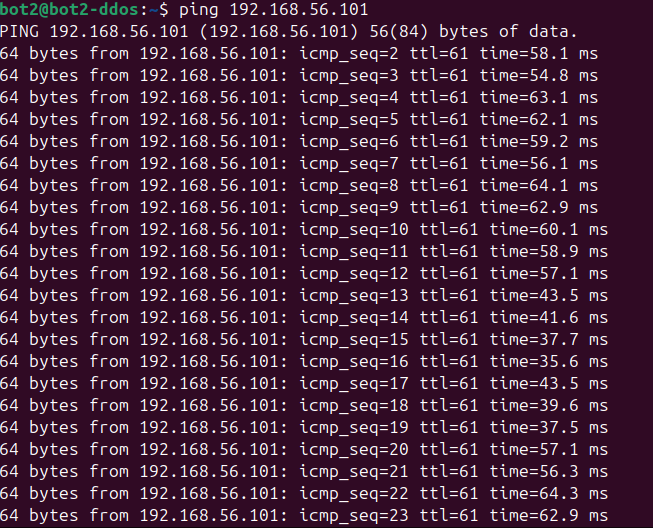
\includegraphics[width=0.8\linewidth]{thesis/bot2ToServer.png}
    \caption{Ping to check connection between bot2 and server}
    \label{fig:enter-label}
\end{figure}
\begin{figure}[htp]
    \centering
    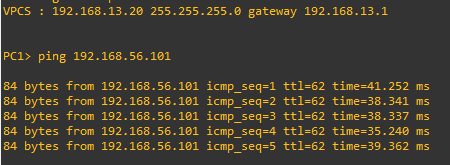
\includegraphics[width=0.8\linewidth]{thesis/pc1ToServer.png}
    \caption{Ping to check connection between pc1 and server}
    \label{fig:enter-label}
\end{figure}
\begin{figure}[!htp]
    \centering
    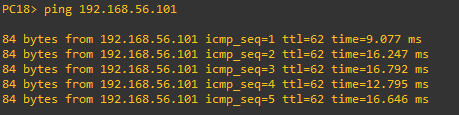
\includegraphics[width=0.8\linewidth]{thesis/pc18ToServer.png}
    \caption{Ping to check connection between pc18 and server}
    \label{fig:enter-label}
\end{figure}
\begin{figure}[!htb]
    \centering
    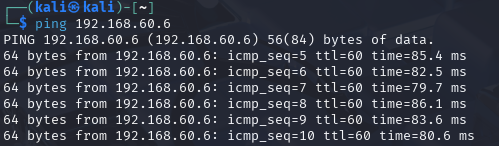
\includegraphics[width=0.8\linewidth]{thesis/kaliToBot1.png}
    \caption{Ping to check connection between attacker machine and bot1}
    \label{fig:enter-label}
\end{figure}
\begin{figure}[!htb]
    \centering
    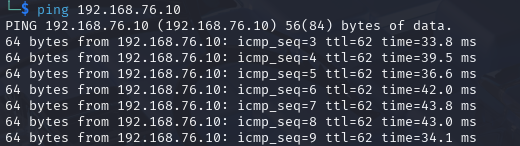
\includegraphics[width=0.8\linewidth]{thesis/kaliToBot2.png}
    \caption{Ping to check connection between attacker machine and bot2}
    \label{fig:enter-label}
\end{figure}
\pagebreak
\section{Methods} 
Overall, the DDoS attack is conducted using an attacker's machine from network 192.168.0.0. When it happens, the attacker machine will send a command to all zombie machines. Assume that the victim's machine has not been infected and the attacker has connection to the victim's machine network. But then the attacker will encounter another issue, the victim's machine has a password. So, on the attacker's machine, we have to trigger the bots using the "ssh-keygen" by setting up SSH key authentication to bypass the bot machine's password. 
\\
To begin, a SSH keypair is created on the attacker's machine (the machine that triggers the bots).
\begin{figure}[h]
    \centering
    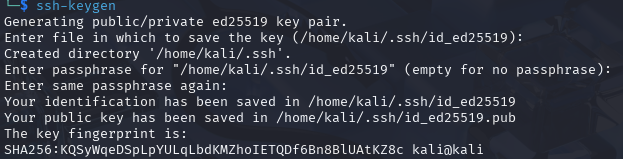
\includegraphics[width=0.8\linewidth]{thesis/ssh-keygen.png}
    \caption{Create SSH key pair on the attacker machine}
    \label{fig:enter-label}
\end{figure}
\\ After doing this, the attacker will have two keys which are public and private keys.
\begin{figure}[!htb]
    \centering
    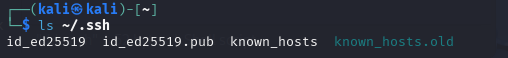
\includegraphics[width=0.8\linewidth]{thesis/2keys.png}
    \caption{The two keys}
    \label{fig:enter-label}
\end{figure}
\\
The attacker then proceeds to share the public keys with bots by copying them using the command "ssh-copy-id bot1@192.168.60.6". It will then ask the password one last time and install the public key in "/.ssh/authorized \textunderscore keys" on the bots.
\begin{figure}[!htb]
    \centering
    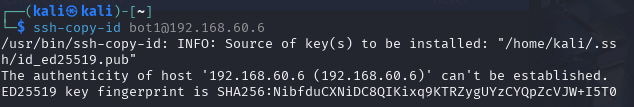
\includegraphics[width=0.8\linewidth]{thesis/ssh-copy-id-1.png}
    \caption{Copy the attacker's public key to bot1}
    \label{fig:enter-label}
\end{figure}
\\
Next, copy the key to bot2's machine.
\begin{figure}[!htb]
    \centering
    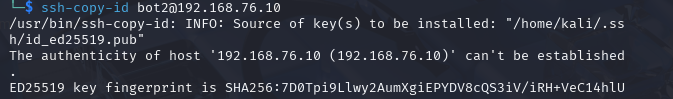
\includegraphics[width=0.8\linewidth]{thesis/ssh-copy-id-2.png}
    \caption{Copy the attacker's public key to bot2}
    \label{fig:enter-label}
\end{figure}
\\ After this, we can launch an attack by ssh to zombie machines without typing in any password. For the attack tool, we use hping3, which is a network tool capable of sending ICMP, UDP, TCP to display target replies like ping does with ICMP replies. Before being able to attack, the attacker must first copy attack script (ddos.sh) to zombie machines.
\\
By using the following scp command, the attacker can securely copy the attack file called "ddos.sh" to the bot machines in whatever directory the attacker wants to.
\begin{lstlisting}[language=bash,caption={Command to copy ddos.sh file to bot1}]
$ scp ddos.sh bot1@192.168.60.6:/home/bot1
\end{lstlisting}
Do the same thing with bot2.
\begin{lstlisting}[language=bash,caption={Command to copy ddos.sh file to bot2}]
$ scp ddos.sh bot2@192.168.76.10:/home/bot2
\end{lstlisting}
After that, the ddos files are in the zombie machines.
\begin{figure}[htb]
    \centering
    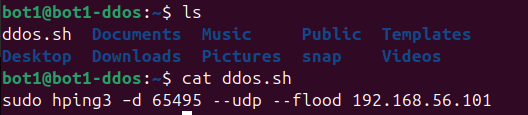
\includegraphics[width=0.8\linewidth]{thesis/bot1AfterCopy.png}
    \caption{Successfully copy ddos.sh to bot1}
    \label{fig:enter-label}
\end{figure}
\pagebreak
\begin{figure}[!htb]
    \centering
    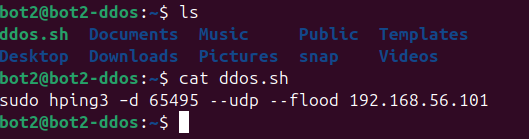
\includegraphics[width=0.8\linewidth]{thesis/bot2AfterCopy.png}
    \caption{Successfully copy ddos.sh to bot2}
    \label{fig:enter-label}
\end{figure}
\\ The next step is to install passwordless sudo by ssh to each bot then go to the visudo by typing.
\begin{lstlisting}[language=bash,caption={Setting up passwordless sudo}]
 $sudo visudo
\end{lstlisting}
\begin{figure}[!htb]
    \centering
    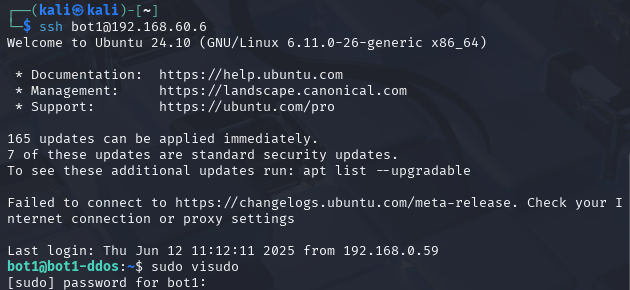
\includegraphics[width=0.8\linewidth]{thesis/visudo.png}
    \caption{Edit sudoers file}
    \label{fig:enter-label}
\end{figure}
\\ Add the following line at the end.
\begin{lstlisting}[language=bash,caption={Setting up passwordless sudo on bot1}]
bot1 ALL=(ALL) NOPASSWD:ALL
\end{lstlisting}
\begin{figure}[!htb]
    \centering
    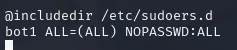
\includegraphics[width=0.5\linewidth]{thesis/passwordless.png}
    \caption{Add passwordless command}
    \label{fig:enter-label}
\end{figure}
\\ 
Repeat the same process for bot2, add the command to sudoers file of bot2.
\begin{lstlisting}[language=bash,caption={Setting up passwordless sudo on bot2}]
bot2 ALL=(ALL) NOPASSWD:ALL
\end{lstlisting}
\\
The attacker then needs a script to command all bots to execute the file ddos.sh. The file is called "start\_attack.sh".
\begin{lstlisting}[language=bash,caption={Content of start\_attack.sh}]
#!/bin/bash

# List of bots 
BOTS=("bot1@192.168.60.6" "bot2@192.168.76.10")

for BOT in "${BOTS[@]}"
do
    echo "Triggering attack on $BOT..."
    ssh -o StrictHostKeyChecking=no ${BOT} "sudo bash \$HOME/ddos.sh" &
done

echo "All bots triggered!"
\end{lstlisting}
Now we must implement a way to stop the attack. With the SSH key pairs we already created, we will utilize it to kill the process of hping3, thus, will stop the attack.
\begin{lstlisting}[language=bash,caption={Content of stop\_attack.sh}]
#!/bin/bash

# List of bots 
BOTS=("bot1@192.168.60.6" "bot2@192.168.76.10")

for BOT in "${BOTS[@]}"
do
    echo "Stopping attack on $BOT"
    ssh "$BOT" 'pkill -f hping3'
done
\end{lstlisting}
\section{Suricata Configuration}
In order to allow Suricata to run successfully in the Intrusion Prevention System (IPS) mode, it will be essential to set the core parameters properly through the suricata.yaml configuration file. This file controls the Suricata behavior on managing network traffic, interfaces, processing packets, matching rules, and output behavior \cite{lane2024defensive}.
\\
In this section, essential Suricata settings to be applied in project work will be discussed, especially the ones that concern af-packet, NFQUEUE, and IPS mode enable.
\subsection{Suricata.yaml File Details}
The suricata.yaml file is a comprehensive configuration file defaultly placed at /etc/suricata/suricata.yaml. It consists of multiple sections:
\begin{itemize}
    \item General settings \\
    Logging, default directories, run modes.
    \item Capture interfaces \\
    How Suricata reads packets (af-packet, pcap, NFQUEUE).
    \item Detection engine \\
    Rule sets, thresholds, and flow tracking.
    \item Output \\
    Logging, alert files, EVE JSON.
    \item Advanced options \\
     CPU affinity, threading, and memory settings.
\end{itemize}
"af-packet" is a Linux kernel-based packet capture method that enables high-performance packet acquisition. It is used when Suricata is in IDS (Intrusion Detection System) mode, listening passively on a network interface.
\begin{lstlisting}[language=bash,caption={Part contains af-packet}]
af-packet:
  - interface: enp0s3
    threads: auto
    cluster-id: 99
    cluster-type: cluster_flow
    defrag: yes
\end{lstlisting}
Configuration explain:
\begin{itemize}
    \item interface \\
    The NIC interface Suricata listens on (In this experiment is enp0s3).
    \item cluster-id \\
    Must be unique if multiple interfaces are used.
    \item cluster-type \\
    Determines how traffic is distributed across threads.
    \item defrag \\
    Enables IP defragmentation for accurate detection.
\end{itemize}
\subsection{NFQUEUE Configuration}
In IPS mode, Suricata runs in NFQUEUE mode which is a Linux application that enables the iptables to forward traffic to the userspace (Suricata) to examine and make a verdict decision. Here is the NFQUEUE setting in suricata.yaml
\begin{lstlisting}[language=bash,caption={Part contains NFQUEUE}]
nfq:
  mode: accept
  repeat-mark: 1
  route-queue: 0
\end{lstlisting}
Explaination:
\begin{itemize}
    \item mode: accept \\
    Packets are accepted unless dropped by a rule.
    \item route-queue \\
    Specifies which NFQUEUE ID Suricata should listen to.
\end{itemize}
\subsection{Logs and Alerts}
Suricata logs IPS activities to files such as:
\begin{itemize}
    \item /var/log/suricata/fast.log\\
    Quick summary alerts.
    \item /var/log/suricata/eve.json\\
    Detailed structured logs.
\end{itemize}
In order to view logs, we use the following command.
\begin{lstlisting}[language=bash,caption={View Suricata logs}]
$ sudo tail -f /var/log/suricata/fast.log
\end{lstlisting}
Here is what Suricata logs look like.
\begin{figure}[!htb]
    \centering
    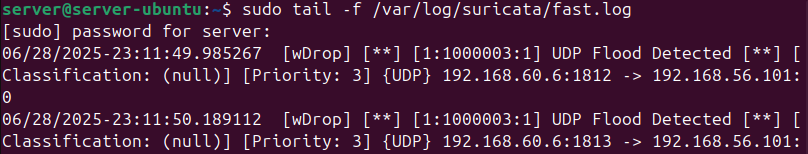
\includegraphics[width=0.8\linewidth]{thesis/suricataLog.png}
    \caption{Suricata Logs}
    \label{fig:enter-label}
\end{figure}